
\documentclass[a4paper]{article} %
\usepackage{graphicx,amssymb} %

\textwidth=15cm \hoffset=-1.2cm %
\textheight=25cm \voffset=-2cm %

\pagestyle{empty} %

\date{} %

\def\keywords#1{\begin{center}{\bf Keywords}\\{#1}\end{center}} %



% Please, do not change any of the above lines




\usepackage{epstopdf}



\begin{document}

% Type down your paper title
\title{Structured Sparsity in Numerical Optimisation}

% Authors
\author{Matteo Frigo \\ %
       University of C\^ote d'Azur, Inria (France) \\
       Athena Project-Team \\ \\ % Affiliation 1
       \tt{matteo.frigo@inria.fr} % Only one corresponding e-mail
       }%


\maketitle

\thispagestyle{empty}



% The abstract

\begin{abstract}
A significant portion of the challenges in applied mathematics can be formulated as a convex optimisation problem. The question about how to solve this problems is the first that will be addressed in this talk; in particular we will focus on the class of proximal splitting methods, which provides us many useful tools for solving non-smooth optimisation problems. We will also explore the concepts of sparsity and structured sparsity, showing how they turn out to be a valuable tool for designing specific models in medical imaging. The final part of the talk will be devoted to the case of brain connectivity mapping, which will give us the occasion to study a real world application of structured sparsity in numerical optimisation.
\end{abstract}

\keywords{Structured Sparsity, Convex Optimisation, Proximal Splitting Methods, Brain Connectivity}

%\begin{center}
%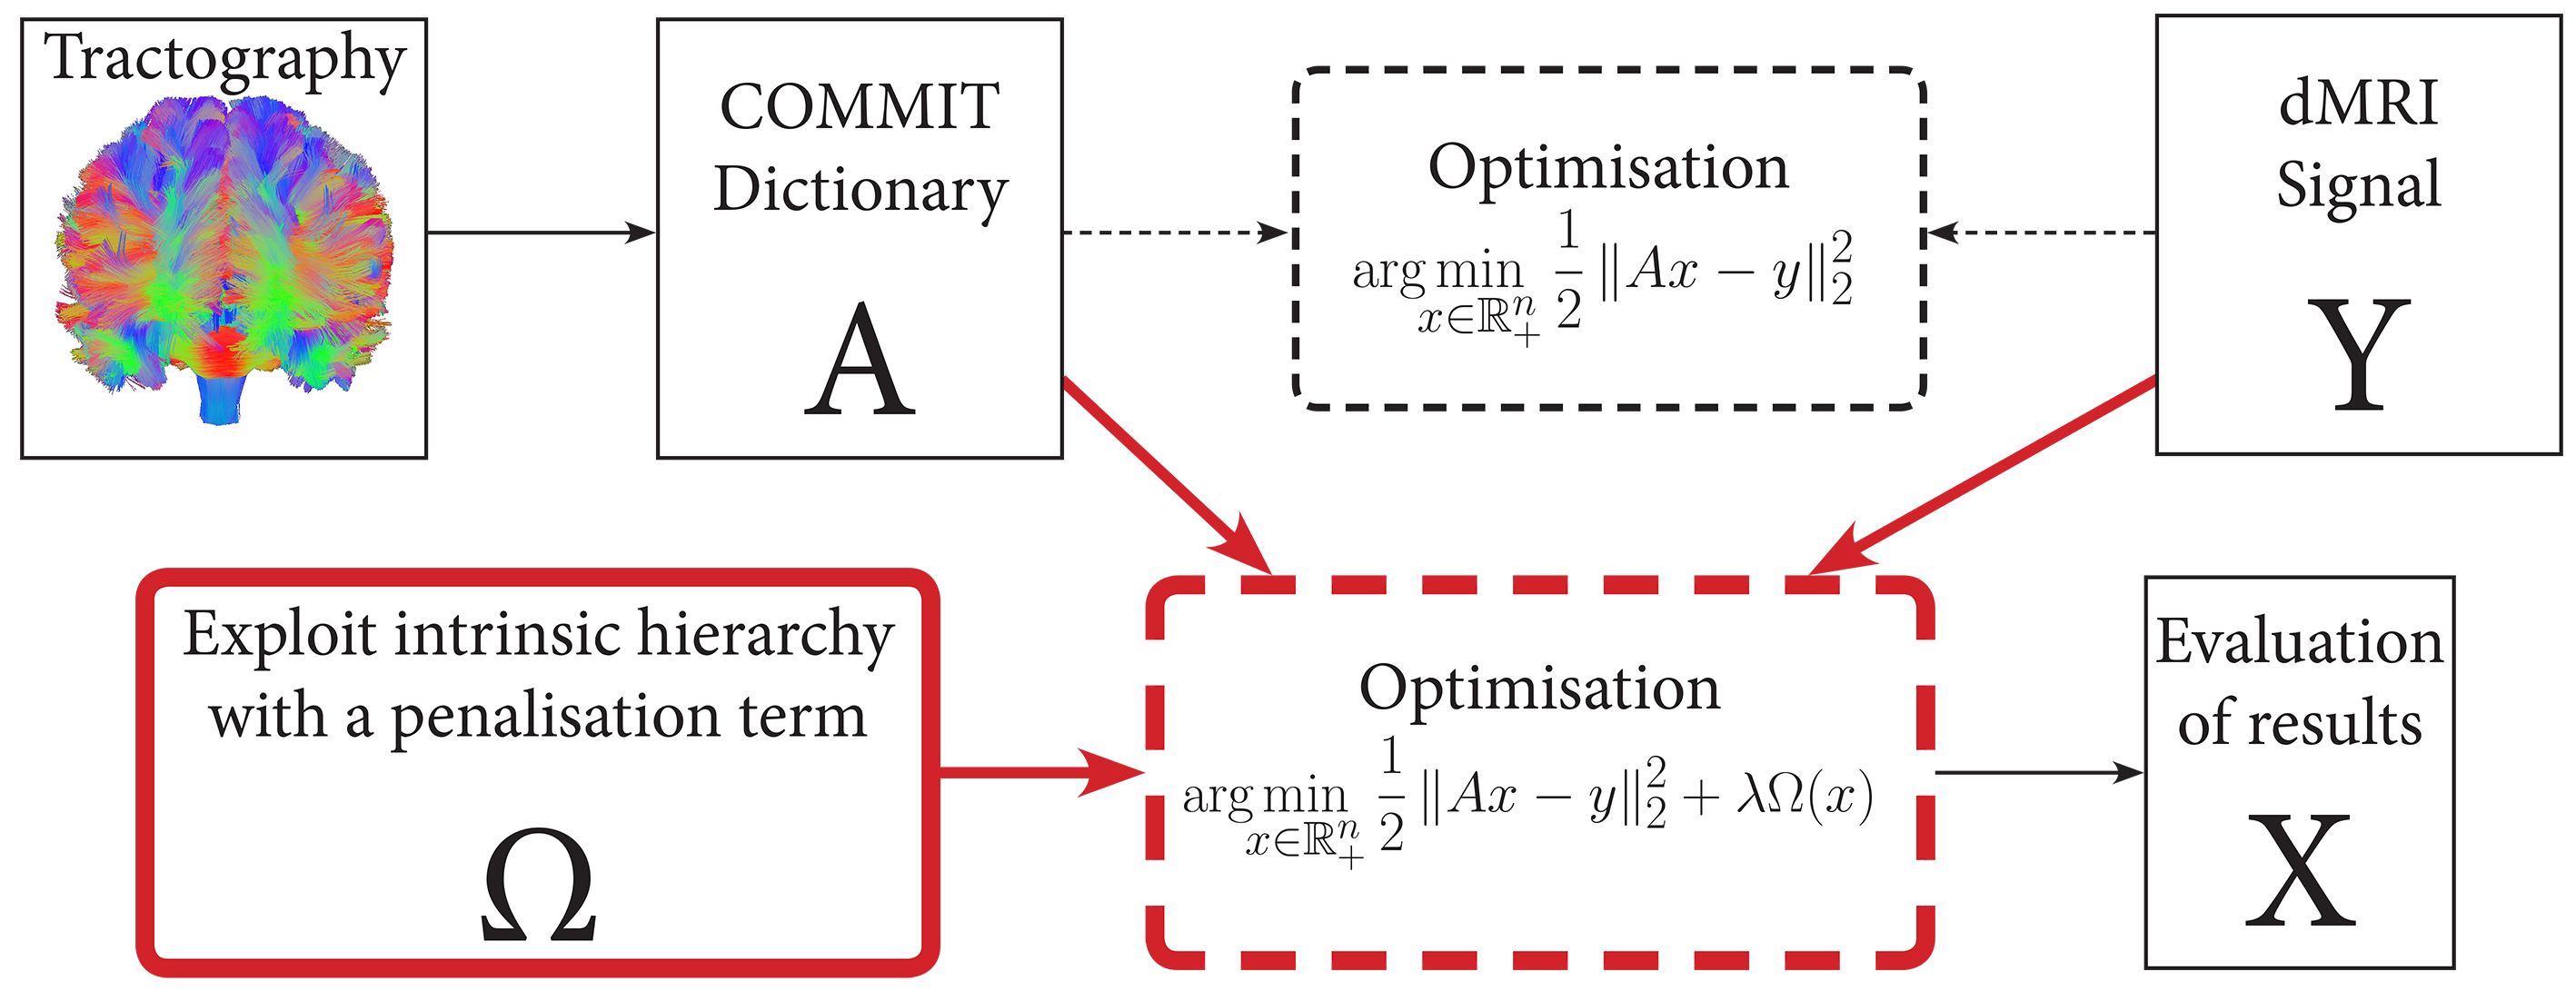
\includegraphics[width=.8\textwidth]{diagram}
%\end{center}

\vfill
\noindent This work has received funding from the European Research Council (ERC) under the European Union's Horizon 2020 research and innovation program (ERC Advanced Grant agreement No 694665 : CoBCoM - Computational Brain Connectivity Mapping).
\begin{center}

\includegraphics[height=1cm,keepaspectratio]{flag_yellow_high}
\qquad

\includegraphics[height=1cm,keepaspectratio]{erc_logo}
\qquad
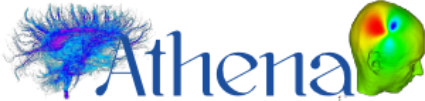
\includegraphics[height=1cm,keepaspectratio]{athena-logo}
\qquad

\includegraphics[height=1cm,keepaspectratio]{logo_inria}
\end{center}




% \section{Introduction}






\end{document}
